% Gemini theme
% https://github.com/anishathalye/gemini

\documentclass[final,12pt]{beamer}

% ====================
% Packages
% ====================

\usepackage[T1]{fontenc}
\usepackage{lmodern}
% Dimensions: 4'-by-3.5' in cm
% Cannot exceed 6'-by-4'=182.88 x 121.92 cm
% Note: LMSAL printer width is 44''=111.76 cm
\usepackage[size=custom,width=121.92,height=108.76,scale=1.0]{beamerposter}
\usetheme{gemini}
\usecolortheme{labsix}
\usepackage{graphicx}
\usepackage{booktabs}
\usepackage{tikz}
\usepackage{pgfplots}
\usepackage{multicol}
\usepackage[numbers]{natbib}
\usepackage{import}
\usepackage{siunitx}
\usepackage{caption}
\usepackage{amsmath}
\usepackage{mathrsfs}

% hack to use the caption package with beamer
\makeatletter
\let\@@magyar@captionfix\relax
\makeatother

% Include all PythonTeX related stuff
%spell-checker: disable
%  PythonTeX Configuration

\usepackage{pythontex}
\usepackage{pgf}
\usepackage{import}
% % % % % % % % % % % % % % % % % % % % % % % % % % % % % % % % % %
% PythonTeX Bug Fix % % % % % % % % % % % % % % % % % % % % % % % %
% % % % % % % % % % % % % % % % % % % % % % % % % % % % % % % % % % 
% pytexbug fix for context in customcode.
\makeatletter
\renewenvironment{pythontexcustomcode}[2][begin]{%
	\VerbatimEnvironment
	\Depythontex{env:pythontexcustomcode:om:n}%
	\ifstrequal{#1}{begin}{}{%
		\ifstrequal{#1}{end}{}{\PackageError{\pytx@packagename}%
			{Invalid optional argument for pythontexcustomcode}{}
		}%
	}%
	\xdef\pytx@type{CC:#2:#1}%
	\edef\pytx@cmd{code}%
	% PATCH \def\pytx@context{}%
	\pytx@SetContext
	% END PATCH
	\def\pytx@group{none}%
	\pytx@BeginCodeEnv[none]}%
{\end{VerbatimOut}%
\setcounter{FancyVerbLine}{\value{pytx@FancyVerbLineTemp}}%
\stepcounter{\pytx@counter}%
}%
\makeatother
% % % % % % % % % % % % % % % % % % % % % % % % % % % % % % % % % %

\setpythontexcontext{textwidth=\the\textwidth,columnwidth=\the\columnwidth,figurewidth=\the\textwidth}

%% Setup PythonTeX and TeXFigure
\begin{pythontexcustomcode}{py}
import os
import pathlib
import sys
sys.path.append('./python/')

import texfigure
pytex.formatter = texfigure.repr_latex_formatter

import numpy as np
import matplotlib
import matplotlib.pyplot as plt
import matplotlib.colors
import seaborn
import sunpy.map
import astropy.units as u
import astropy.constants as const
from astropy.visualization import ImageNormalize, AsinhStretch, SqrtStretch, LogStretch

# Define color palettes
PALETTE = seaborn.color_palette('colorblind', 100)
DEEP_PALETTE = seaborn.color_palette('deep', 100)
# Register colormaps
from colormaps import *

# Set some plot styling here
normalsize = 24.88  # it'd be better to set this automatically...
preamble = [
	r'\usepackage{siunitx}',
	r'\DeclareSIUnit[number-unit-product={}]\erg{erg}',
	r'\DeclareSIUnit[number-unit-product={}]\dn{DN}',
	r'\DeclareSIUnit[number-unit-product={}]\pixel{pixel}',
	r'\DeclareSIUnit[number-unit-product={}]\photon{photon}',
	r'\DeclareSIUnit[number-unit-product={}]\gauss{G}',
	r'\DeclareSIUnit[number-unit-product={}]\dyne{dyne}',
]
rc = {
	'pgf.preamble': preamble,
	'pgf.rcfonts': False,
	'pgf.texsystem': 'lualatex',
	'text.latex.preamble': preamble,
	'text.usetex': True,
	'font.family': 'sans-serif',
	'font.serif': [], # Leave blank to inherit from document
	'font.sans-serif': [], # Leave blank to inherit from document
	'font.monospace': [], # Leave blank to inherit from document
	'font.size': normalsize,
	'axes.titlesize': normalsize,
	'axes.labelsize': 0.9 * normalsize,
	'axes.labelpad': 5,
	'legend.fontsize': 0.75 * normalsize,
	'xtick.labelsize': 0.75 * normalsize,
	'ytick.labelsize': 0.75 * normalsize,
	'xtick.major.pad': 5,
	'xtick.minor.pad': 5,
	'ytick.major.pad': 5,
	'ytick.minor.pad': 5,
	'xtick.direction': 'in',
	'ytick.direction': 'in',
	'savefig.dpi': 200,
	'savefig.format': 'pdf',
	'savefig.bbox': 'tight',
}
texfigure.configure_latex_plots(pytex, **rc)

\end{pythontexcustomcode}


% Lengths
% If you have N columns, choose \sepwidth and \colwidth such that
% (N+1)*\sepwidth + N*\colwidth = \paperwidth
\newlength{\sepwidth}
\newlength{\colwidth}
\setlength{\sepwidth}{0.025\paperwidth}
\setlength{\colwidth}{0.3\paperwidth}

% Other macros
\DeclareMathOperator*{\argmax}{arg\,max}
\newcommand{\fourier}[1]{\mathscr{F}\left\{#1\right\}}
\newcommand{\inversefourier}[1]{\mathscr{F}^{-1}\left\{#1\right\}}
\newcommand{\angstrom}{\textup{\AA}}
\newcommand{\separatorcolumn}{\begin{column}{\sepwidth}\end{column}}

\title{The Sun at Scale: Interactive Analysis of SDO Data on HPC Platforms with Dask}

\author{Will Barnes \inst{1}\textsuperscript{,}\inst{2}\textsuperscript{,}\inst{3}\textsuperscript{\inst{\dagger}} \and
        Mark Cheung \inst{2} \and
        Monica Bobra \inst{3} \and
        Arthur Amezcua \inst{3} \and
        Herbert Yeung \inst{4}\textsuperscript{,}\inst{5} \and
        Stuart Mumford \inst{6}
}

\institute[]{
  \inst{1} Bay Area Environmental Research Institute \samelineand
  \inst{2} Lockheed Martin Solar and Astrophysics Laboratory \samelineand
  \inst{3} W. W. Hansen Experimental Physics Laboratory, Stanford University \and
  \inst{4} Arctic Slope Regional Corporation \samelineand
  \inst{5} NASA Ames Research Center \samelineand
  \inst{6} University of Sheffield \samelineand
  \inst{\dagger} Visiting Postdoctoral Scholar
}

\footercontent{
  \href{https://gitlab.com/wtbarnes/aia-on-pleiades}{gitlab.com/wtbarnes/aia-on-pleiades} \hfill
  AGU Fall Meeting 2019 --- San Francisco, CA USA --- 12 December 2019 \hfill
  \href{mailto:barnes@baeri.org}{barnes@baeri.org}
}

\begin{document}

% Logos
% LMSAL logo goes here
\addtobeamertemplate{headline}{} 
{
    \begin{tikzpicture}[remember picture,overlay] 
      \node [anchor=north west, inner sep=3cm] at ([xshift=-1.3cm,yshift=4cm]current page.north west)     {
\includegraphics[width=20cm]{../../logos/baeri-logo.png}};
    \end{tikzpicture} 
}
\addtobeamertemplate{headline}{} 
{
    \begin{tikzpicture}[remember picture,overlay] 
      \node [anchor=north east, inner sep=3cm] at ([xshift=-8cm,yshift=1.3cm]current page.north east)     {\includegraphics[height=8cm]{../../logos/SU_Seal_Red_R_Small.eps}};
    \end{tikzpicture} 
}
\addtobeamertemplate{headline}{} 
{
    \begin{tikzpicture}[remember picture,overlay] 
      \node [anchor=north east, inner sep=3cm] at ([xshift=0cm,yshift=2cm]current page.north east)     {
\includegraphics[height=9cm]{../../logos/sunpy_powered_logo.png}}; 
    \end{tikzpicture} 
}
%\addtobeamertemplate{headline}{} 
%{
%    \begin{tikzpicture}[remember picture,overlay] 
%      \node [anchor=north east, inner sep=3cm] at ([xshift=0cm,yshift=1.4cm]%current page.north east)     {\includegraphics[height=8.5cm]{../../%logos/agu_centennial.png}}; 
%    \end{tikzpicture} 
%}

% Setup TeXFigure environment
% spell-checker: disable %
\begin{pycode}[manager]
manager = texfigure.Manager(
    pytex, './',
    python_dir='python',
    fig_dir='figures',
    data_dir='data',
)
\end{pycode}
% spell-checker: enable %

\begin{frame}[fragile,t]
\begin{columns}[T]
\separatorcolumn

\begin{column}{\colwidth}

  \begin{block}{The Solar Dynamics Observatory}
    \begin{columns}
      \begin{column}{0.6667\columnwidth}
        \begin{itemize}
          \item The \alert{\textit{Solar Dynamics Observatory} (SDO)} \citep{pesnell_solar_2012} helps us understand the structure and generation of the Sun's magnetic field, how energy is stored and released in the solar corona, and how that energy is released into the heliosphere
          \item SDO carries three scientific instruments
          \begin{itemize}
            \item \alert{\textit{Atmospheric Imaging Assembly} (AIA)} -- EUV and UV emission in corona and chromosphere
            \item \alert{\textit{Helioseismic and Magnetic Imager} (HMI)} -- magnetic and velocity fields at the solar surface
            \item \textit{Extreme Ultraviolet Variability Experiment} (EVE) -- disk-integrated spectral irradiance
          \end{itemize}
          \item AIA and HMI data publicly available and served to the community by \alert{\textit{Joint Science Operations Center} (JSOC)} \citep{couvidat_observables_2016} at Stanford University 
        \end{itemize}
      \end{column}
      \begin{column}{0.3\columnwidth}
        \begin{figure}
          \centering
          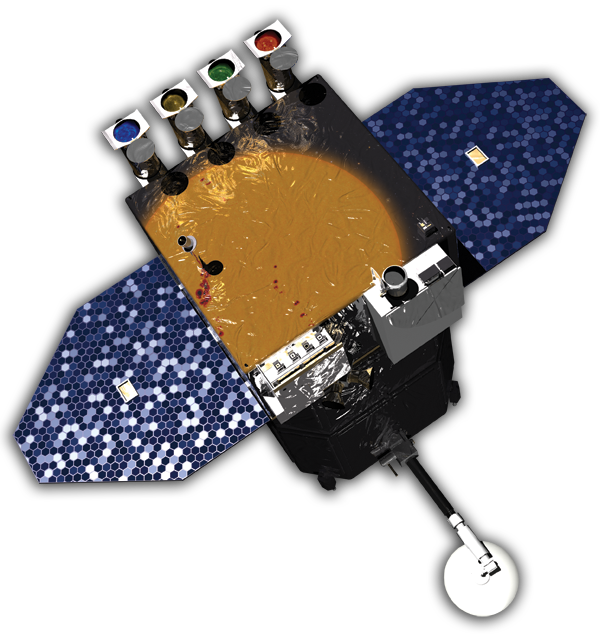
\includegraphics[width=\columnwidth]{figures/sdo.png}
        \end{figure}
      \end{column}
    \end{columns}
    \begin{itemize}
      \item Since May 2010, AIA has delivered nearly continuous \alert{4K resolution} images of the Sun in \alert{7 EUV wavelengths} at a \alert{cadence of 12 s}
      \begin{itemize}
        \item \alert{2 TB of data per day}
        \item Current \alert{total of 15 PB} spread out over \alert{$\approx200\times10^6$ files} for AIA alone
        \item Data volume is growing daily!
      \end{itemize}
      \item \alert{\textbf{Problem:}} Current software infrastructure and data access model inhibit users from taking full advantage of SDO data using modern computing capabilities
      \item \alert{\textbf{Goal:}} Demonstrate need for a platform for \alert{scalable, interactive analysis of SDO data} using high performance computing (HPC) and open-source scientific software in Python
    \end{itemize}
  \end{block}

  \begin{block}{An Interactive and Scalable Python Workflow for SDO Data}

    \begin{itemize}
      \item Current SDO data workflow: make a query against JSOC using IDL, Python (via the \texttt{drms} Python module \citep{glogowski_drms_2019}), or via a web interface
      \item Each time step and wavelength stored in a separate compressed FITS file, downloaded serially to the user's local workstation
    \end{itemize}

    \begin{figure}
      \centering
      \def\svgwidth{0.7\columnwidth}
      \import{figures/}{old_workflow.pdf_tex}
      %\resizebox{0.65\columnwidth}{!}{\import{figures/}{old_workflow.pdf_tex}}
    \end{figure}

    \begin{itemize}
      \item This workflow presents several limitations:
      \begin{itemize}
        \item Data transfer of many files over HTTP can be very slow (e.g. $>1$ day for 12 hours of AIA data in 6 EUV wavelengths)
        \item High volume of requests stresses infrastructure of data provider
        \item Requires large disk storage on user end
        \item Single user workstations likely have limited computing capability
      \end{itemize}
      \item Proposed solution: \alert{move data source to a shared, hosted computing environment} 
    \end{itemize}

    \begin{figure}
      \centering
      \def\svgwidth{0.8\columnwidth}
      \import{figures/}{new_workflow.pdf_tex}
      %\resizebox{0.65\columnwidth}{!}{\import{figures/}{old_workflow.pdf_tex}}
    \end{figure}

    \begin{itemize}
      \item Perform interactive analysis on \alert{NASA Pleiades HPC} resources via Jupyter notebook interface
      \item All data on shared filesystem--only reduced science results transferred over network
      \item Analyze data using modern Python stack for astronomy, e.g. \texttt{astropy} \citep{the_astropy_collaboration_astropy_2018}, \texttt{sunpy} \citep{sunpy_community_sunpypython_2015}, \texttt{ndcube}
      \item \alert{Parallelize computations over $>10^3$ cores} using \texttt{dask} library for distributed computing \citep{rocklin_dask_2015}
    \end{itemize}

  \end{block}

  \begin{block}{Current Infrastructure}
    \begin{itemize}
      \item Data Record Management Service (DRMS) software installed on NASA Pleiades hardware
      \item Modified \texttt{drms} Python code such that \alert{queries return file paths on shared Lustre filesystem}
      \item No bulk data download--data is fetched ``as needed'' based on science use cases
      \item Computation scaled out over compute nodes using Dask ``meta scheduler'' on top of existing PBS scheduling software (see \href{https://github.com/dask/dask-jobqueue}{github.com/dask/dask-jobqueue})
      \item Running on underutilized legacy Merope cluster -- 1,792 repurposed Intel Westmere processors each with \alert{12 cores, 48 GB memory}
      \item Provided access to the entire Merope cluster, \alert{estimate that current level 1 AIA data set could be processed to level 1.5 in just over 2 days}
      \item See \href{https://gitlab.com/wtbarnes/aia-on-pleiades}{gitlab.com/wtbarnes/aia-on-pleiades} for extended documentation and example notebooks
    \end{itemize}
  \end{block}

\end{column}

\separatorcolumn

\begin{column}{\colwidth}
  \begin{block}{Application: Tracking Global EUV Waves}

% spell-checker: disable %
\begin{pycode}[manager]
fig = plt.figure(figsize=texfigure.figsize(
    pytex,
    scale=0.8,
    height_ratio=0.3,
))

m_before = sunpy.map.Map(os.path.join(manager.data_dir, 'running_ratio_171_before.fits'))
m_during = sunpy.map.Map(os.path.join(manager.data_dir, 'running_ratio_171_during.fits'))
m_after = sunpy.map.Map(os.path.join(manager.data_dir, 'running_ratio_171_after.fits'))
# Before
ax = fig.add_subplot(131, projection=m_before)
m_before.plot(axes=ax,
       norm=ImageNormalize(vmin=-0.125, vmax=0.125),
       title=False,
       cmap='better_RdBu')
ax.grid(False)
ax.coords[0].set_axislabel(' ')
ax.coords[1].set_axislabel(' ')
ax.coords[0].set_ticklabel_visible(False)
ax.coords[1].set_ticklabel_visible(False)
# During
ax = fig.add_subplot(132, projection=m_during)
m_during.plot(axes=ax,
       norm=ImageNormalize(vmin=-0.125, vmax=0.125),
       title=False,
       cmap='better_RdBu')
ax.grid(False)
ax.coords[0].set_axislabel(' ')
ax.coords[1].set_axislabel(' ')
ax.coords[0].set_ticklabel_visible(False)
ax.coords[1].set_ticklabel_visible(False)
# After
ax = fig.add_subplot(133, projection=m_after)
m_after.plot(axes=ax,
       norm=ImageNormalize(vmin=-0.125, vmax=0.125),
       title=False,
       cmap='better_RdBu')
ax.grid(False)
ax.coords[0].set_axislabel(' ')
ax.coords[1].set_axislabel(' ')
ax.coords[0].set_ticklabel_visible(False)
ax.coords[1].set_ticklabel_visible(False)
plt.subplots_adjust(0.01)
tfig = manager.save_figure('euv-wave-ratio', fext='.pdf')
tfig.caption = r'Log of the running ratio of the 171 \angstrom{} intensity for a window of 240 s before (\textbf{left}), during (\textbf{middle}), and after (\textbf{right}) the 2017 September 10 flaring event. Red indicates areas where the plasma is being heated and blue indicates areas where the plasma is being cooled.'
tfig.figure_width = r'\columnwidth'
\end{pycode}
\py[manager]|tfig|
% spell-checker: enable %

\begin{itemize}
    \item Global EUV waves, triggered by flares/CMEs, can be used to probe the global structure of the corona -- \alert{requires full-disk observations}
    \item \citet{liu_truly_2018} used running ratio calculation in AIA 171, 193, 211 \angstrom{} to track global EUV wave from the 2017 September 10 X8.2+ flaring event
    \item Registered and stacked 2 hours of full-resolution, full-disk AIA 171 \angstrom{} observations into coordinate-aware \texttt{ndcube} objects
    \item \alert{Computed log running ratio in parallel for full 2 hour period in $<2$ minutes using \texttt{dask}}
    \item Allows for quick visualization of high time resolution dynamics across the full disk
\end{itemize}

\end{block}

  \begin{block}{Example: Time Lag Analysis}

How can time lag analysis be used to understand coronal heating \citet{viall_evidence_2012}

Describe time lag mathematically \citet{barnes_understanding_2019}

Show time lag map for a single channel pair

Show scaling of time lag calculation with number of cores

\end{block}
\end{column}

\separatorcolumn

\begin{column}{\colwidth}
  \begin{block}{Example: Automatic Detection of Sunspots}

Describe STARA algorithm \citet{watson_modelling_2009}

What we did, why would we want to do this

How fast was it (compare to serial computation)? 

Read in data, resampled images, and performed automatic sunspot detection using STARA on 1 image per day for the entire mission and built catalogue of segmented regions in less than 2 minutes using 660 computing cores (55 nodes with 12 cores each)

Show sunspot count as function of time, butterfly diagram, maybe 

% spell-checker: disable %
\begin{pycode}[manager]
# Load table
tab = astropy.table.Table.read(os.path.join(manager.data_dir, 'sunspot_catalogue.fits'))
tab['obstime'] = astropy.time.Time(tab['obstime'])
# Calculate monthly sunpot number
delta_time = tab['obstime'] - tab['obstime'][0]
bin_size = 30*u.day
spots,bins = np.histogram(
    delta_time.to(bin_size.unit).value,
    bins=np.arange(0,(delta_time[-1]+1*u.day).to(bin_size.unit).value, bin_size.value),)
time_spots = (bins[1:] + bins[:-1])/2*u.day + tab['obstime'][0]
kernel = Box1DKernel(6)  # smooth over 6 months because 1 time unit is 30 days
spots_smooth = convolve(spots, kernel)
# Plot
fig = plt.figure(figsize=texfigure.figsize(
    pytex,
    scale=1,
    height_ratio=0.4,
))
# sunspot number
ax = fig.add_subplot(121)
with time_support(simplify=True, format='decimalyear'):
    ax.plot(time_spots, spots,)
    ax.plot(time_spots, spots_smooth)
ax.set_ylabel('Number of Spots (monthly total)');
ax.set_xlabel(f'Time');
ax.set_ylim(0, spots.max()*1.05);
# butterfly diagram
ax = fig.add_subplot(122)
with time_support(simplify=True, format='decimalyear'):
    ax.scatter(tab['obstime'][::10], tab['center_lat'][::10],
    marker='o', alpha=0.1)
ax.axhline(y=0, ls='--', color='k')
ax.axhline(y=-30, ls=':',color='k')
ax.axhline(y=+30, ls=':',color='k')
ax.set_ylim(-40,40)
ax.set_xlabel(f'Time')
ax.set_ylabel(f'Heliographic Latitude [{tab["center_lat"].unit}]');
plt.subplots_adjust(wspace=0.3)
# Save plot
tfig = manager.save_figure('sunspots', fext='.pgf')
tfig.caption = r''
tfig.figure_width = r'0.95\columnwidth'
\end{pycode}
\py[manager]|tfig|
% spell-checker: enable %

\end{block}
  \vspace{-3ex}
  \begin{block}{Application: Calculating Space-Weather Parameters}

\begin{columns}
\begin{column}{0.5\columnwidth}
% spell-checker: disable %
\begin{pycode}[manager]
tab = astropy.table.QTable.read(
    os.path.join(manager.data_dir, 'sharps_unsigned_flux_table.fits'))
tab['time'] = astropy.time.Time(tab['time'], scale='tai')
fig = plt.figure(figsize=texfigure.figsize(
    pytex,
    scale=1,
    height_ratio=1,
))
ax = fig.gca()
with time_support(simplify=True):
    ax.plot(tab['time'], tab['unsigned_flux']/1e22,
            color=PALETTE[0], label='modified')
    ax.plot(tab['time'], tab['unsigned_flux_fits']/1e22,
            color=PALETTE[1], label='original')
ax.set_xlabel(f'Time')
ax.set_ylabel('Total Unsigned Flux [$10^{22}$ Mx]')
ax.legend(loc=2)
tfig = manager.save_figure('sharps-unsigned-flux', fext='.pgf')
tfig.caption = f'Evolution of the total unsigned flux over a period of 7 days starting on {tab["time"][0]} for active region NOAA 11158. The blue curve shows the unsigned flux computed using the modified SHARPs calculation with Dask while the orange curve shows the unsigned flux values extracted from the SHARPs metadata.'
tfig.figure_width = r'\columnwidth'
\end{pycode}
\py[manager]|tfig|
% spell-checker: enable %
\end{column}

\begin{column}{0.5\columnwidth}
\begin{itemize}
    \item Space-weather HMI Active Region Patches \citep[SHARPS,][]{bobra_helioseismic_2014} data products include keywords describing various physical parameters of active regions (e.g. total unsigned flux)
    \item \alert{Scalar parameters often used in machine learning context} \citep[e.g.][]{bobra_solar_2015, zheng_solar_2019} because they can be accessed without downloading image data
    \item Recalculating SHARP features for varying input parameters \alert{may influence predictions of machine learning models}--important to understand why and how
    \item Recalculated total unsigned flux for active region NOAA 11158 over 7 days in $\approx30$ s in parallel via \texttt{dask} and \texttt{numpy}
    \item \alert{Estimate that every SHARP parameter for all $~2.7\times10^6$ images could be recalculated in a matter of days using $10^3$ cores}
\end{itemize}
\end{column}
\end{columns}

\end{block}

  \begin{block}{Conclusions and Future Work}
    \begin{columns}
    \begin{column}{0.75\columnwidth}
      \begin{itemize}
        \item Demonstrated viability of SDO analysis at scale using NASA Pleiades and Dask for wide variety of science applications
        \item Data locality combined with scalable computing \alert{critical to maximizing scientific return of the SDO dataset}
        \item \textbf{\alert{Recommendation:}} a hosted computing platform for heliophysics -- already adopted by other disciplines (e.g. Pangeo, LSST)
        \item Cloud/HPC increasingly important as data sets grow in size and complexity (e.g. DKIST)
        \item \alert{Open development of Python analysis tools is crucial to this effort} 
        \item \textbf{Scan QR code for screencasts of example applications}
      \end{itemize}
    \end{column}
    \begin{column}{0.25\columnwidth}
      \begin{figure}
        \centering
        
\includegraphics[width=\columnwidth]{figures/qr-code.eps}
      \end{figure}
    \end{column}
    \end{columns}
  \end{block}

  \begin{block}{References}
    \scriptsize

    We thank Wei Liu, Ignacio Ugarte-Urra, and Fraser Watson for their help in developing example use cases. We also thank Jeff Becker and Bob Ciotti for their assistance with the Pleiades HPC system. This poster was typeset using Lua\TeX and Python\TeX \citep{poore_pythontex_2015}.

      \begin{multicols}{2}
        \bibliographystyle{aasjournal.bst}
        \bibliography{references.bib}
      \end{multicols}

  \end{block}

\end{column}

\separatorcolumn
\end{columns}
\end{frame}

\end{document}
